\chapter{Mod�le du syst�me}

Etudions maintenant les possibilit�s d'utilisation du futur logiciel.

\section{Cas d'utilisation}




\section{Diagramme de classes}

Notre  projet  s'architecture autour  d'une  classe principale  nomm�e
Agent.  Le diagramme  UML  de  classes est  disponible  sur la  figure
\ref{fig:diagramme_classes}.

\begin{figure}[ht]
  \centering
  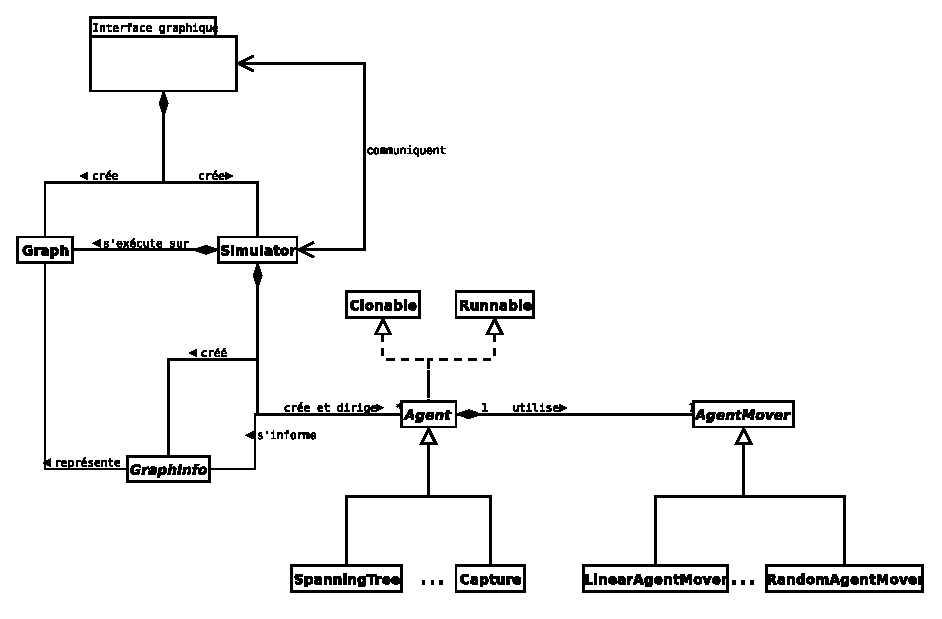
\includegraphics[width=14cm]{classes}  
  \caption{Diagramme de classes}
  \label{fig:diagramme_classes}
\end{figure}


\subsection{La classe Agent et ses sous-classes}

La  classe  Agent  impl�mente  toutes les  m�thodes  n�cessaires  pour
faciliter  le  travail du  futur  d�veloppeur  d'agents mobiles.   Les
m�thodes  seront  d�crites dans  la  partie  \ref{sec:api}  � la  page
\pageref{sec:api}. \\

De fa�on g�n�rale, on peut  trouver des m�thodes d'informations sur le
graphe, des m�thodes  de gestion de propri�t�s (au  niveau des sommets
et des portes), des m�thodes de d�placements et de clonage.\\

Le futur d�veloppeur devra,  pour impl�menter ses agents, sous-classer
cette classe Agent et impl�menter la m�thode abstraite suivante : \\

\begin{description}
\item[init] Utilis�e pour impl�menter le code g�n�ral de l'algorithme.
  C'est cette m�thode qui sera lanc�e lorsque l'agent sera ex�cut�.
\end{description}

\subsection{La classe AgentMover}

AgentMover  est  une classe  qui  a pour  but  d'apporter  un type  de
d�placement aux  agents. Certains type de  d�placements seront fournis
par \visidia et d'autres  pourront �tre impl�ment�s par le d�veloppeur
lorsqu'il en ressentira le besoin. \\

Lors de l'impl�mentation d'un agent, le d�veloppeur devra utiliser les
m�thodes  ``move'' pour  se d�placer.  Ces m�thodes  sont en  fait des
appels cach�s aux m�thodes de AgentMover. \\

Pour d�velopper  un nouveau  type de d�placement,  l'utilisateur devra
donc impl�menter  une nouvelle sous classe de  AgentMover et red�finir
la m�thode ``findNextDoor''.

%% Local Variables:
%% mode: latex
%% coding: latin-1
%% TeX-master: "main"
%% End:
